\documentclass[12pt,letterpaper]{article}

\usepackage{arxiv}

\usepackage[utf8]{inputenc} % allow utf-8 input
\usepackage[T1]{fontenc}    % use 8-bit T1 fonts
\usepackage{hyperref}       % hyperlinks
\usepackage{url}            % simple URL typesetting
\usepackage{booktabs}       % professional-quality tables
\usepackage{amsfonts}       % blackboard math symbols
\usepackage{nicefrac}       % compact symbols for 1/2, etc.
\usepackage{microtype}      % microtypography
\usepackage{lipsum}
\usepackage{graphicx}	% Including figure files
\usepackage{mathtools}  %loads amsmath as well
\usepackage{amssymb}	% Extra maths symbols
\usepackage[english]{babel}
\usepackage{float}
\usepackage{bm}
\usepackage{indentfirst}
\usepackage{tikz}
\usetikzlibrary{positioning}
\usepackage{pgfplots}
\usepackage{color,soul}
%\pgfplotsset{compat=1.12}
\definecolor{mygray}{RGB}{125,125,125}
\definecolor{myred}{RGB}{255,60,60}
\definecolor{myblue}{RGB}{60,60,255}
\renewcommand{\arraystretch}{1.2}

% potential journals:
    % journal of computational physics
    % computers and fluids
    % international journal for numerical methods in fluids
    % aiaa
    % journal of fluid mechanics

%\title{A Multiresolution Scheme Featuring Fully Adaptive Blocks for Simulating Reactive Flows}
\title{A Multiresolution Scheme for Accelerating High-Order WENO Computations on Adaptive Mesh Refinement Blocks}

\author{
  Brandon Gusto\\
  Department of Scientific Computing\\
  Florida State University\\
  Tallahassee, FL 32306 \\
  \texttt{bgusto@fsu.edu} \\
  %% examples of more authors
  \And
  Tomasz Plewa \\
  Department of Scientific Computing\\
  Florida State University\\
  Tallahassee, FL 32306 \\
  \texttt{tplewa@fsu.edu} \\
}

\begin{document}
\maketitle

\begin{abstract}
    We present a generalization of Harten's original multiresolution scheme for
    simulating reactive flows on logically rectangular block-structured adaptive
    mesh refinement (AMR) grids in one and two dimensions. The scheme addresses
    a major shortcoming of tree-based AMR codes, which is the creation of blocks
    with a low filling factor; that is, many cells in such a block are resolved
    beyond the desired error tolerance, necessitating excessive computational
    resources.  To overcome this issue, we introduce a multiresolution
    representation of the solution, not only to adapt the grid but also to
    adaptively compute fluxes and sources on each block. The scheme recycles
    regularity information obtained by the multiresolution grid adaptation in
    order to select flux and source calculations which may be accurately
    replaced by interpolation from the multiresolution basis. A block which
    employs this scheme is denoted as a fully adaptive block (FAB).  The error
    introduced by this approximation is shown to be of the same order as the
    local truncation error of the reconstruction scheme. Thus the rate of
    convergence of the underlying spatial reconstruction scheme is preserved.
    Additionally with respect to parallel applications, the multiresolution
    transform and computation of fluxes and sources on FABs is asynchronous,
    requiring only one synchronization step which is equivalent to the filling
    of ghost cells for each block. The efficiency of the scheme is demonstrated
    using several one and two-dimensional problems.
\end{abstract}

% keywords can be removed
\keywords{Multiresolution \and Adaptive Mesh Refinement \and Conservation Laws}

\section{Introduction}

    % paragraph introduces the need for spatially adaptive grids
    Fluid flows are often characterized by disparate spatial and temporal length
    scales. Certain features such as turbulence or shocks necessitate
    significantly higher resolution than smooth regions of the flow.  In
    reacting flows, combustion fronts often act in highly localized regions, and
    on very small time scales. Naturally, intense effort has gone into the
    development of methods which employ a multi-scale or adaptive strategy to
    accurately simulate such flows without over-resolving smooth areas of the
    domain.

    % paragraph introducing adaptive mesh refinement as a concept
    The most popular strategy to accurately capture regions of interest in fluid
    simulations is to introduce a non-uniform spatial grid, with higher
    resolution in regions of interest.  Methods which introduce a hierarchy of
    nested grid resolutions are generally described as adaptive mesh refinement
    (AMR) methods. AMR methods rely on estimates of the local truncation error (LTE)
    of the numerical scheme to determine regions where refinement is necessary for solution
    accuracy. Several strategies to approximate the LTE are used (\hl{list
    methods}).
    %\cite{Berger1984}.  Alternate methods include
    %feature-based refinement, and evaluation of gradient information (references
    %here).

    % talk about block-structured AMR
    Regarding the implementation of AMR methods on large parallel computers,
    certain engineering realities have neccessitated the reduction in
    granularity of the adaptive refinement. To use a single computational cell
    as the unit for refinement (i.e. cell-based refinement) introduces a number
    of costly compromises. Firstly, such an adapted grid requires the
    reconstruction method of choice to utilize nonuniform stencils, requiring
    increased computational resources. More significantly, the cell-based
    refinement requires extremely costly data traversal. Traversing tree space
    requires an average $\mathcal{O}(n^d)$ (\hl{confirm this?}) operations. Thus
    most AMR codes make use of some type of block-based approach. Tree-based
    block-structured codes, where each block consists of a fixed number of
    cells, are a very popular choice. These types of approaches are implemented
    in a number of AMR libraries including Paramesh (\hl{cite}), p4est
    (\hl{cite}, and others. This approach allows for simple mesh management
    procedures, and scales well for very large number of processors in parallel.

    % paragraph reviews the work of harten and multiresolution methods
    Alternate approaches to dynamic grid adaptation based on wavelet theory have
    become popular in recent years. The first such effort was introduced in a
    seminal paper by Harten \cite{harten1994}, where a multiresolution
    representation of the discrete solution on a uniform grid was used for
    adaptively computing the divergence of the flux within a finite volume
    framework. Rather than adapt the grid by truncating the wavelet basis, the
    idea was to accelerate the computation of high-order essentially
    non-oscillatory (ENO) schemes using the multiresolution information. Fluxes
    in smooth regions were interpolated from fluxes obtained at interfaces
    corresponding to coarser grid levels. The original scheme was applied solely
    to hyperbolic conservation laws, but was then expanded by Bihari et. al. to
    two-dimensional simulations in (\hl{citation}), followed by the inclusion of
    viscous terms in (\hl{citation}), and then tp source terms in the context of
    reactive flows in (\hl{citation}). These works retained the original flavor
    of Harten's scheme, which was to represent the discrete solution on a
    uniform grid, but uses a multiresolution representation of the solution to
    identify regions where flux (and source term) computations may be avoided.
    The multiresolution transform is obtained by using average-interpolating
    wavelets as basis functions.

    % review the multiresolution-adaptive papers
    Although Harten's original scheme was intended to be an alternative to
    spatially non-uniform grid adaptation, a series of papers have since
    reintroduced this concept of non-uniform grids within the MR framework. Thus
    the AMR approach has been redeveloped but with the refinement criterion
    defined by the MR representation rather than with the traditional metrics
    mentioned previously. The first fully adaptive scheme was presented by Cohen
    et. al. to study hyperbolic conservation laws in two dimensions in
    (\hl{cite}).

\section{Governing Equations and Finite Volume Discretization}

    % describe merging block-structured AMR with Harten's scheme
    In the present work we are interested in numerically solving conservation
    laws of the form
    \begin{equation}
    \begin{cases}
      u_{t} + f(u)_{x} = s(u) \\    
      u(x,0) = u_{0}(x),
    \end{cases}
    \label{claw}
    \end{equation} where $x \in \Omega$, $t \in [t_{0},t_{fin}]$, $u$ represents a conserved quantity, $f(u)$ is the flux
    function, and $s(u)$ is a source term. For the sake of presentation, we let
    the scalar equation (\ref{claw}) stand in for the more complicated systems
    of conversation laws which will be the focus of our applications.  In the
    finite volume formulation, the solution $u(x,t)$ is approximated by volume
    averages defined within each cell $I_{i} = \left[ x_{i}-\frac{h}{2},
    x_{i}+\frac{h}{2} \right]$ in the computational domain.  The cell width $h$
    is determined by the number of cells, $N$, and the size of the domain
    $\Omega \in \left[a,b\right]$.  The cell averages are given by
    \begin{equation}
        u_{i}(t) = \frac{1}{h} \int_{x_{i-1/2}}^{x_{i+1/2}} u(\xi,t) d \xi,
    \end{equation}
    where for convenience we use $i \pm 1/2$ as subscripts to
    indicate the left and right interfaces of the target cell (i.e.
    $x_{i+1/2} =
    x_{i} + \frac{h}{2}$). The governing equations are cast into the
    semi-discrete conservative form,
    \begin{equation}
        \frac{du_{i}(t)}{dt} = -\frac{1}{h} \left( \hat{f}_{i+1/2} -
        \hat{f}_{i-1/2} \right),
        \label{ode}
    \end{equation}
    where the numerical flux is evaluated as
    \begin{equation}
        \hat{f}_{i\pm1/2} = \hat{f}(u^{-}_{i\pm1/2}, u^{+}_{i\pm1/2}).
    \end{equation}
    The states $u^{-}_{i\pm1/2}$ and $u^{+}_{i\pm1/2}$ indicate the approximate
    value of the quantity $u$ immediately to the left and right of the cell
    interface $x_{i\pm1/2}$. These values are reconstructed from a stencil of
    cell averages using weighted essentially non-oscillatory schemes of
    variable order.

    \subsection{Reconstruction with WENO Polynomials}

    \subsection{Time Integration}

        % define evolution operator as in domingues2008
        Once the system of ordinary differential equations (\ref{ode}) is
        established, the objective is to integrate them forward in time. In our
        implementation we use a second-order explicit Runge-Kutta scheme to
        advance. This is summarized by
        \begin{equation}
            \bm{u}^{n+1} = \bm{E} \bm{u}^{n},
        \end{equation}
        where $\bm{E}$ represents the nonlinear evolution operator, and codifies the
        temporal and spatial discretizations.

\section{Harten's Multiresolution Scheme on a Uniform Grid}

    % describe overview of transform, and average-interpolating wavelets
    We present here a review of Harten's multiresolution method for adaptive
    flux computations within the original context of uniform, one-dimensional
    grids. This is necessary to illustrate the extension of the scheme to
    block-structured AMR grids. The multiresolution approach is based on a
    hierarchy of nested discretizations on the domain of interest, $\Omega$.
    The hierarchy consists of grids at a coarsest level $l=1$ to a finest grid
    $l=L$, where any two adjacent levels differ by a refinement factor of two.
    The grids are defined by
    \begin{equation}
        \bm{\mathcal{G}}_{l} = \left\{ x_{i}^{l} \right\}_{i=0}^{N_{l}}, \text{ }
        \text{ } \text{ } \text{ } x_{i}^{l} = i \cdot h_{l}, \text{ }
        \text{ } h_{l} = 2^{L-l} \cdot h_{L}, \text{ } \text{ } N_{l} = N_{L}
        / 2^{L-l},
    \end{equation}
    where $h_{l}$ and $N_{l}$ denote the cell width and number of cells,
    respectively, on level $l$. We denote the finest grid by
    $\bm{\mathcal{G}}_{L}$. denote the index space of cells on each level
    of the hierarchy by $\bm{\mathcal{I}}^{l} = (1,\dots,N^{l})$.

    \subsection*{Encoding}

        % describe the prediction operator, and detail coefficients
        Given a vector of discrete cell averages at the finest resolution,
        $\bm{u}^{L}$, the multiresolution representation is obtained by the
        following operations:
        \begin{enumerate}
            \item[] \textit{Split:} The cells at grid level $l$ are split into
                even and odd sets, $\bm{\mathcal{I}}_{even}^{l}$ and
                $\bm{\mathcal{I}}_{odd}^{l}$, based on their indices.
            \item[] \textit{Project:} The cells at level $l+1$ are projected
                by means of volume averaging, onto the coarser grid
                level $l$. The projection is defined by a linear operator
                which performs the mapping $\bm{P}_{l+1}^{l} : \bm{u}^{l+1}
                \mapsto \bm{u}^{l}$. 
            \item[] \textit{Predict}: A stencil of cell averages $i \in
                \bm{\mathcal{I}}_{odd}^{l}$ are predicted by an
                average-interpolating polynomial based on cells at level $l-1$.
                Thus, the prediction operator performs the mapping
                $\bm{P}_{l-1}^{l} : \bm{u}^{l-1} \mapsto \bm{u}^{l}$. 
        \end{enumerate}
        The projection preserves averages at the finer level, by design, and in
        the context of uniform grids is the simple averaging of parent cells,
        \begin{equation}
            u^{l}_{i} = \left( \bm{P}_{l+1}^{l} \bm{u}^{l+1} \right)_{i} = \frac{1}{2} ( u^{l+1}_{2i-1} + u^{l+1}_{2i} ), \text{ }
            \text{ } \text{ } \text{ } \forall i \in \bm{\mathcal{I}}^{l}.
        \end{equation}
        The prediction operator is defined by a unique average-interpolating
        polynomial to predict, based on a stencil of cell-averages at grid level
        $l$, the odd cell averages at the finer level level $l+1$. The
        prediction mapping is performed using the following centered
        interpolants,
        \begin{equation}
            \tilde{u}_{i}^{l} = \left( \bm{P}_{l-1}^{l} \bm{u}^{l-1}
            \right)_{i} = 
            \begin{cases}
                u_{i/2}^{l-1} - \sum_{p=1}^{s} \gamma_{p} \left( u^{l-1}_{i/2-p} -
                u^{l-1}_{i/2+p} \right), \text{ } \text{ } \text{ } \forall
                i \in \bm{\mathcal{I}}_{even}^{l} \\
                u_{(i+1)/2}^{l-1} + \sum_{p=1}^{s} \gamma_{p} \left(
                u^{l-1}_{(i+1)/2-p} - u^{l-1}_{(i+1)/2+p} \right), \text{ }
                \text{ } \text{ } \forall i \in \bm{\mathcal{I}}_{odd}^{l}
            \end{cases}
        \end{equation}
        The coefficients $\gamma_{i}$ are supplied in Table
        (\ref{coeff1}). The order of accuracy of each interpolant is $r=2s+1$.
        \begin{table}[]
            \center
            \begin{tabular}{|l|l|l|l|l|}
            \hline
                order    & $\gamma_{1}$ & $\gamma_{2}$ & $\gamma_{3}$ & $\gamma_{4}$ \\ \hline
                3 & 1/8          & 0            & 0            & 0            \\ \hline
                5 & -22/128      & 3/128        & 0            & 0            \\ \hline
                7 & 0            & 0            & 0            & 0            \\ \hline
                9 & 0            & 0            & 0            & 0            \\ \hline
            \end{tabular}
            \label{coeff1}
            \caption{For the derivation of these coefficients, the reader is referred to Appendix (\hl{ref}).}
        \end{table}
        Once the prediction is made, the difference information on level $l$ is
        obtained by computing the detail coefficient as
        \begin{equation}
            d^{l}_{i} = u^{l+1}_{2i} - \tilde{u}^{l+1}_{2i}, \text{ } \text{ }
            \text{ } \text{ } \forall i \in \bm{\mathcal{I}}^{l}.
        \end{equation}
        for each cell.  The encoding procedure is complete when the detail
        coefficients have been computed on all levels $l=0,\dots,L-1$.  The
        entire procedure can be succinctly written in terms of a matrix-vector
        operation to yield the multiresolution representation of the data,
        $u_{M}^{L}$, as
        \begin{equation}
            \bm{u}^{L}_{M} = \bm{M} \bm{u}^{L} = \left( \bm{d}^{L-1}, \bm{d}^{L-2},
            \dots, \bm{d}^{0}, \bm{u}^{0} \right)^{T}.
        \end{equation}
        Here the multiresolution operator $\bm{M}$ contains the prediction
        operation and subsequent detail coefficient calculation for each cell
        on each level of the hierarchy.

    \subsection*{Truncation}

        % describe truncation proceudure
        Once the difference information has been computed, compression of the
        fine-grid cell averages $\bm{u}^{L}$ is obtained by truncating
        coefficients whose magnitude is below a prescribed level-dependent
        threshold, $\varepsilon_{l}$.  In \cite{harten1994} the following
        threshold is proposed
        \begin{equation}
            \varepsilon_{l} = \varepsilon / 2^{L-l}.
        \end{equation}
        The detail coefficients are truncated according to
        \begin{equation}
            \tilde{d}^{l}_{i} =
                \begin{cases}
                    d^{l}_{i}, \text{ } \text{if} \text{ } |d^{l}_{i}| > \varepsilon_{l} \\
                    0, \text{ } \text{if} \text{ } |d^{l}_{i}| \leq
                    \varepsilon_{l},
                \end{cases}
        \end{equation}
        producing the following approximate representation,
        \begin{equation}
            \tilde{\bm{u}}^{L}_{M} = T_{\varepsilon}(\bm{u}^{L}_{M}) = \left(
            \tilde{\bm{d}}^{L-1}, \tilde{\bm{d}}^{L-2},
            \dots, \tilde{\bm{d}}^{0}, \bm{u}^{0} \right)^{T}.
        \end{equation}
        
    \subsection*{Decoding}

        % describe decoding
        The fine-grid solution is reconstructed by computing from levels
        $l=1,\dots,L-1$ the following
        \begin{align}
            u_{2i}^{l+1} & = d_{i}^{l} + \tilde{u}_{2i}^{l+1} \\
            u_{2i-1}^{l+1} & = 2 u_{i}^{l} - u_{2i}^{l+1},
        \end{align}
        for each cell on the level.  If the detail coefficients are truncated
        below a nonzero $\varepsilon$, the discrete representation becomes
        \begin{equation}
            \bm{u}^{L}_{\varepsilon} \approx \bm{M}^{-1} \tilde{\bm{u}}^{L}_{M}.
        \end{equation}


    \subsection*{Adaptive Calculation of Fluxes and Sources}

        % dicuss computation of fluxes and sources
        Once the detail coefficients have been obtained, the MR scheme
        proceeds by setting a threshold $\varepsilon$ and truncating coefficients
        which have an absolute value below the threshold. Lastly, the inverse
        transform then starts from grid $l=L$ and at each interface either
        computes fluxes using the fine-grid scheme, or interpolates them using
        the MR basis. The fluxes are interpolated by
        \begin{equation}
            \tilde{f}_{2i+1}^{l-1} \approx \sum_{p=1}^{s+1} \beta_{p} \left(
            \hat{f}^{l}_{i-p+1} + \hat{f}^{l}_{i+p} \right),
        \end{equation}
        \begin{table}[]
            \center
            \begin{tabular}{|l|l|l|l|l|}
            \hline
                order    & $\beta_{1}$ & $\beta_{2}$ & $\beta_{3}$ & $\beta_{4}$ \\ \hline
                3 & 9/16         & -1/16        & 0            & 0            \\ \hline
                5 & 0            & 0            & 0            & 0            \\ \hline
                7 & 0            & 0            & 0            & 0            \\ \hline
                9 & 0            & 0            & 0            & 0            \\ \hline
            \end{tabular}
            \label{coeff1}
            \caption{}
        \end{table}
        where the interpolants are of degree $2s+1$. The coefficients for
        various degrees of polynomial interpolants are shown in Table (ref).
        The process repeats until all fluxes are either computed or
        interpolated on the fine grid $l=0$.

    \subsection*{Error Analysis}

\section{Asynchronous Fully Adaptive Block Scheme}

    \subsection*{Block-Structured Mesh Adaptation}
    % two main issues: no jump greater than one refinement level, and no
    % incomplete trees
    We define a mask $\bm{\mathcal{M}}(\varepsilon)$.

    % illustration of parallel encoding
    \begin{figure}[H]
        \center
        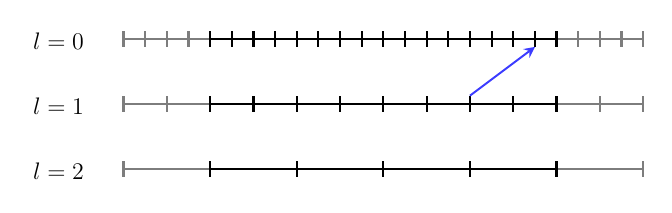
\begin{tikzpicture}[thick,scale=0.275, every node/.style={scale=0.6}]

    % variables
    \def\xl{-8.0}
    \def\xr{8.0}
    \def\y{0.0}
    \def\yy{-3.0}
    \def\yyy{-6.0}
    \def\ts{0.75}
    \def\op{0.35}
    \def\fx{0.15}
    
    % draw ghost cells
    \draw [mygray] (\xl-4,\y+\ts/2) --(\xr+4,\y+\ts/2);
    \draw [mygray] (\xl-4,\yy+\ts/2) --(\xr+4,\yy+\ts/2);
    \draw [mygray] (\xl-4,\yyy+\ts/2) --(\xr+4,\yyy+\ts/2);
    \draw [mygray] (\xl-1.0,\y) --(\xl-1.0,\y+\ts);
    \draw [mygray] (\xr+1.0,\y) --(\xr+1.0,\y+\ts);
    \draw [mygray] (\xl-2.0,\y) --(\xl-2.0,\y+\ts);
    \draw [mygray] (\xr+2.0,\y) --(\xr+2.0,\y+\ts);
    \draw [mygray] (\xl-3.0,\y) --(\xl-3.0,\y+\ts);
    \draw [mygray] (\xr+3.0,\y) --(\xr+3.0,\y+\ts);
    \draw [mygray] (\xl-4.0,\y) --(\xl-4.0,\y+\ts);
    \draw [mygray] (\xr+4.0,\y) --(\xr+4.0,\y+\ts);

    % ghost cells at level l=1
    \draw [mygray] (\xl-2.0,\yy) --(\xl-2.0,\yy+\ts);
    \draw [mygray] (\xr+2.0,\yy) --(\xr+2.0,\yy+\ts);
    \draw [mygray] (\xl-4.0,\yy) --(\xl-4.0,\yy+\ts);
    \draw [mygray] (\xr+4.0,\yy) --(\xr+4.0,\yy+\ts);

    % level l=2
    \draw [mygray] (\xl-4.0,\yyy) --(\xl-4.0,\yyy+\ts);
    \draw [mygray] (\xr+4.0,\yyy) --(\xr+4.0,\yyy+\ts);

    % draw grids
    \draw (\xl,\y+\ts/2) --(\xr,\y+\ts/2);
    \draw (\xl,\yy+\ts/2) --(\xr,\yy+\ts/2);
    \draw (\xl,\yyy+\ts/2) --(\xr,\yyy+\ts/2);
    
    % draw cells for max level
    \draw (\xl,\y) --(\xl,\y+\ts);
    \draw (\xl+1.0,\y) --(\xl+1.0,\y+\ts);
    \draw (\xl+2.0,\y) --(\xl+2.0,\y+\ts);
    \draw (\xl+3.0,\y) --(\xl+3.0,\y+\ts);
    \draw (\xl+4.0,\y) --(\xl+4.0,\y+\ts);
    \draw (\xl+5.0,\y) --(\xl+5.0,\y+\ts);
    \draw (\xl+6.0,\y) --(\xl+6.0,\y+\ts);
    \draw (\xl+7.0,\y) --(\xl+7.0,\y+\ts);
    \draw (\xl+8.0,\y) --(\xl+8.0,\y+\ts);
    \draw (\xl+9.0,\y) --(\xl+9.0,\y+\ts);
    \draw (\xl+10.0,\y) --(\xl+10.0,\y+\ts);
    \draw (\xl+11.0,\y) --(\xl+11.0,\y+\ts);
    \draw (\xl+12.0,\y) --(\xl+12.0,\y+\ts);
    \draw (\xl+13.0,\y) --(\xl+13.0,\y+\ts);
    \draw (\xl+14.0,\y) --(\xl+14.0,\y+\ts);
    \draw (\xl+15.0,\y) --(\xl+15.0,\y+\ts);
    \draw (\xl+16.0,\y) --(\xl+16.0,\y+\ts);
    
    % lower level cells
    \draw (\xl,\yy) --(\xl,\yy+\ts);
    \draw (\xl+2.0,\yy) --(\xl+2.0,\yy+\ts);
    \draw (\xl+4.0,\yy) --(\xl+4.0,\yy+\ts);
    \draw (\xl+6.0,\yy) --(\xl+6.0,\yy+\ts);
    \draw (\xl+8.0,\yy) --(\xl+8.0,\yy+\ts);
    \draw (\xl+10.0,\yy) --(\xl+10.0,\yy+\ts);
    \draw (\xl+12.0,\yy) --(\xl+12.0,\yy+\ts);
    \draw (\xl+14.0,\yy) --(\xl+14.0,\yy+\ts);
    \draw (\xl+16.0,\yy) --(\xl+16.0,\yy+\ts);
    
    % even lower level cells
    \draw (\xl,\yyy) --(\xl,\yyy+\ts);
    \draw (\xl+4.0,\yyy) --(\xl+4.0,\yyy+\ts);
    \draw (\xl+8.0,\yyy) --(\xl+8.0,\yyy+\ts);
    \draw (\xl+12.0,\yyy) --(\xl+12.0,\yyy+\ts);
    \draw (\xl+16.0,\yyy) --(\xl+16.0,\yyy+\ts);
 
    % arrows indicating flux interpolation dependency
    \draw[myblue,->,line width=0.25mm,>=stealth] (\xr-4,\yy+\ts) -- (\xr-1,\y);

    % nodes
    \node at (\xl-7.0,\y+0.25) {\Large $l=0$};
    \node at (\xl-7.0,\yy+0.25) {\Large $l=1$};
    \node at (\xl-7.0,\yyy+0.25) {\Large $l=2$};

\end{tikzpicture}

        \caption{A block of consisting of $N^{0} = 16$ cells is shown. Four
        ghost cells are included on each end of the block, allowing the
        multiresolution decomposition to descend two levels (to grid level
        $l=2$). Interpolation stencils for the computation of detail
        coefficients at levels $l=1, l=2$ are shown, indicating the need for ghost cells.}
    \end{figure}
    % illustration amr block tree structure
    \begin{figure}[H]
        \center
        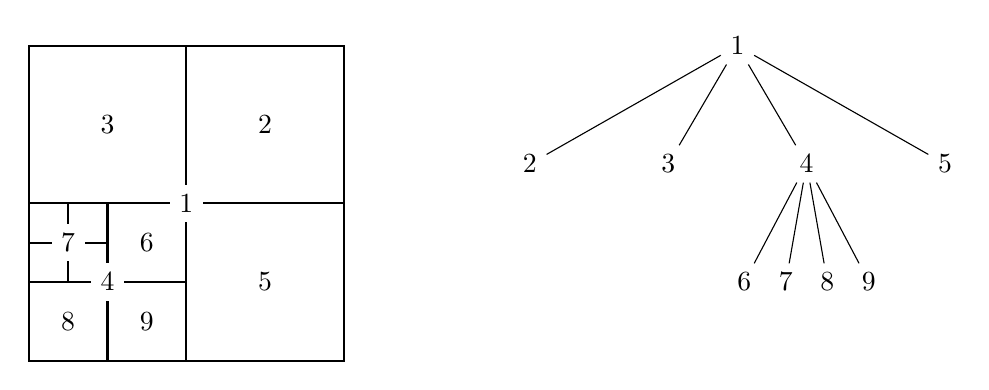
\begin{tikzpicture}[sibling distance=5em,every node/.style = {shape=rectangle,align=center,top color=white}]

    % draw amr blocks
    \draw [thick] (0,0) rectangle (4,4);
    \draw [thick] (2,2) rectangle (4,4);
    \draw [thick] (0,0) rectangle (2,2);
    \draw [thick] (0,0) rectangle (1,1);
    \draw [thick] (1,1) rectangle (2,2);
    \draw [thick] (0,1) rectangle (0.5,1.5);
    \draw [thick] (0.5,1.5) rectangle (1,2);

    % block labels
    \node [shape=rectangle,align=center] at (2,2) {1};
    \node [shape=rectangle,align=center] at (3,3) {2};
    \node [shape=rectangle,align=center] at (1,3) {3};
    \node [shape=rectangle,align=center] at (1,1) {4};
    \node [shape=rectangle,align=center] at (3,1) {5};
    \node [shape=rectangle,align=center] at (1.5,1.5) {6};
    \node [shape=rectangle,align=center] at (0.5,1.5) {7};
    \node [shape=rectangle,align=center] at (0.5,0.5) {8};
    \node [shape=rectangle,align=center] at (1.5,0.5) {9};

    \node at (9,4) {1}
        child { node {2} }
        child { node {3} }
        child { node {4}[sibling distance=1.5em,every node/.style = {shape=rectangle,align=center,top color=white}]
            child { node {6} }
            child { node {7} }
            child { node {8} }
            child { node {9} } }
        child { node {5} };

\end{tikzpicture}

        \caption{}
    \end{figure}

    % pseudocode of algorithm

    % illustration of parallel issue
    \begin{figure}[H]
        \center
        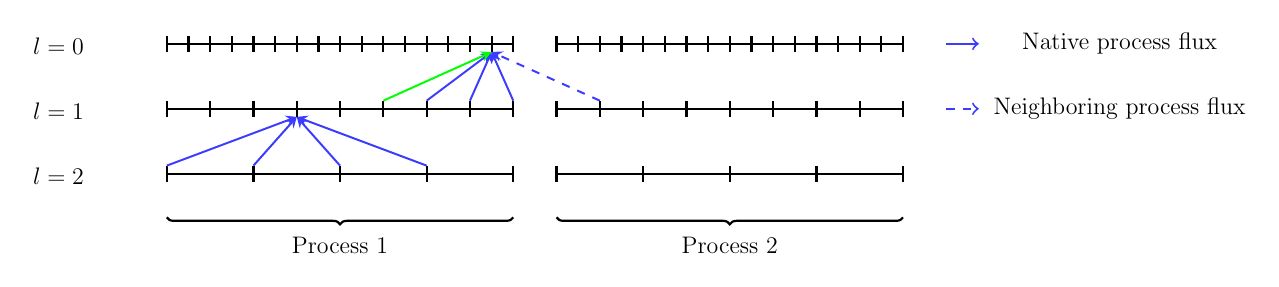
\begin{tikzpicture}[thick,scale=0.275, every node/.style={scale=0.6}]

    % variables
    \def\xl{-8.0}
    \def\xr{8.0}
    \def\y{0.0}
    \def\yy{-3.0}
    \def\yyy{-6.0}
    \def\ts{0.75}
    \def\op{0.35}
    \def\fx{0.15}
    
    % draw grids
    \draw (\xl,\y+\ts/2) --(\xr,\y+\ts/2);
    \draw (\xl,\yy+\ts/2) --(\xr,\yy+\ts/2);
    \draw (\xl,\yyy+\ts/2) --(\xr,\yyy+\ts/2);
    
    % draw cells for max level
    \draw (\xl,\y) --(\xl,\y+\ts);
    \draw (\xl+1.0,\y) --(\xl+1.0,\y+\ts);
    \draw (\xl+2.0,\y) --(\xl+2.0,\y+\ts);
    \draw (\xl+3.0,\y) --(\xl+3.0,\y+\ts);
    \draw (\xl+4.0,\y) --(\xl+4.0,\y+\ts);
    \draw (\xl+5.0,\y) --(\xl+5.0,\y+\ts);
    \draw (\xl+6.0,\y) --(\xl+6.0,\y+\ts);
    \draw (\xl+7.0,\y) --(\xl+7.0,\y+\ts);
    \draw (\xl+8.0,\y) --(\xl+8.0,\y+\ts);
    \draw (\xl+9.0,\y) --(\xl+9.0,\y+\ts);
    \draw (\xl+10.0,\y) --(\xl+10.0,\y+\ts);
    \draw (\xl+11.0,\y) --(\xl+11.0,\y+\ts);
    \draw (\xl+12.0,\y) --(\xl+12.0,\y+\ts);
    \draw (\xl+13.0,\y) --(\xl+13.0,\y+\ts);
    \draw (\xl+14.0,\y) --(\xl+14.0,\y+\ts);
    \draw (\xl+15.0,\y) --(\xl+15.0,\y+\ts);
    \draw (\xl+16.0,\y) --(\xl+16.0,\y+\ts);
    
    % lower level cells
    \draw (\xl,\yy) --(\xl,\yy+\ts);
    \draw (\xl+2.0,\yy) --(\xl+2.0,\yy+\ts);
    \draw (\xl+4.0,\yy) --(\xl+4.0,\yy+\ts);
    \draw (\xl+6.0,\yy) --(\xl+6.0,\yy+\ts);
    \draw (\xl+8.0,\yy) --(\xl+8.0,\yy+\ts);
    \draw (\xl+10.0,\yy) --(\xl+10.0,\yy+\ts);
    \draw (\xl+12.0,\yy) --(\xl+12.0,\yy+\ts);
    \draw (\xl+14.0,\yy) --(\xl+14.0,\yy+\ts);
    \draw (\xl+16.0,\yy) --(\xl+16.0,\yy+\ts);
    
    % even lower level cells
    \draw (\xl,\yyy) --(\xl,\yyy+\ts);
    \draw (\xl+4.0,\yyy) --(\xl+4.0,\yyy+\ts);
    \draw (\xl+8.0,\yyy) --(\xl+8.0,\yyy+\ts);
    \draw (\xl+12.0,\yyy) --(\xl+12.0,\yyy+\ts);
    \draw (\xl+16.0,\yyy) --(\xl+16.0,\yyy+\ts);
    
    % curly brace
    \draw[decoration={brace,mirror,raise=5pt},decorate]
        (\xl,\yyy-1.0) -- node[below=10pt] {\Large Process 1}(\xr,\yyy-1.0);

    % arrows indicating flux interpolation dependency
    \draw[myblue,->,line width=0.25mm,>=stealth] (\xr-4,\yy+\ts) -- (\xr-1,\y);
    \draw[myblue,->,line width=0.25mm,>=stealth] (\xr-2,\yy+\ts) -- (\xr-1,\y);
    \draw[myblue,->,line width=0.25mm,>=stealth] (\xr,\yy+\ts) -- (\xr-1,\y);
    \draw[myblue,dashed,->,line width=0.25mm,>=stealth] (\xr+4,\yy+\ts) -- (\xr-1,\y);
    \draw[green,->,line width=0.25mm,>=stealth] (\xr-6,\yy+\ts) -- (\xr-1,\y);

    \draw[myblue,->,line width=0.25mm,>=stealth] (\xr-16,\yyy+\ts) -- (\xr-10,\yy);
    \draw[myblue,->,line width=0.25mm,>=stealth] (\xr-12,\yyy+\ts) -- (\xr-10,\yy);
    \draw[myblue,->,line width=0.25mm,>=stealth] (\xr-8,\yyy+\ts) -- (\xr-10,\yy);
    \draw[myblue,->,line width=0.25mm,>=stealth] (\xr-4,\yyy+\ts) --(\xr-10,\yy);

    % nodes
    \node at (\xl-5.0,\y+0.25) {\Large $l=0$};
    \node at (\xl-5.0,\yy+0.25) {\Large $l=1$};
    \node at (\xl-5.0,\yyy+0.25) {\Large $l=2$};

    % draw process 2 grid
    \def\xl{10.0}
    \def\xr{26.0}
    \draw (\xl,\y+\ts/2) --(\xr,\y+\ts/2);
    \draw (\xl,\yy+\ts/2) --(\xr,\yy+\ts/2);
    \draw (\xl,\yyy+\ts/2) --(\xr,\yyy+\ts/2);
    
    % draw cells for max level
    \draw (\xl,\y) --(\xl,\y+\ts);
    \draw (\xl+1.0,\y) --(\xl+1.0,\y+\ts);
    \draw (\xl+2.0,\y) --(\xl+2.0,\y+\ts);
    \draw (\xl+3.0,\y) --(\xl+3.0,\y+\ts);
    \draw (\xl+4.0,\y) --(\xl+4.0,\y+\ts);
    \draw (\xl+5.0,\y) --(\xl+5.0,\y+\ts);
    \draw (\xl+6.0,\y) --(\xl+6.0,\y+\ts);
    \draw (\xl+7.0,\y) --(\xl+7.0,\y+\ts);
    \draw (\xl+8.0,\y) --(\xl+8.0,\y+\ts);
    \draw (\xl+9.0,\y) --(\xl+9.0,\y+\ts);
    \draw (\xl+10.0,\y) --(\xl+10.0,\y+\ts);
    \draw (\xl+11.0,\y) --(\xl+11.0,\y+\ts);
    \draw (\xl+12.0,\y) --(\xl+12.0,\y+\ts);
    \draw (\xl+13.0,\y) --(\xl+13.0,\y+\ts);
    \draw (\xl+14.0,\y) --(\xl+14.0,\y+\ts);
    \draw (\xl+15.0,\y) --(\xl+15.0,\y+\ts);
    \draw (\xl+16.0,\y) --(\xl+16.0,\y+\ts);
    
    % lower level cells
    \draw (\xl,\yy) --(\xl,\yy+\ts);
    \draw (\xl+2.0,\yy) --(\xl+2.0,\yy+\ts);
    \draw (\xl+4.0,\yy) --(\xl+4.0,\yy+\ts);
    \draw (\xl+6.0,\yy) --(\xl+6.0,\yy+\ts);
    \draw (\xl+8.0,\yy) --(\xl+8.0,\yy+\ts);
    \draw (\xl+10.0,\yy) --(\xl+10.0,\yy+\ts);
    \draw (\xl+12.0,\yy) --(\xl+12.0,\yy+\ts);
    \draw (\xl+14.0,\yy) --(\xl+14.0,\yy+\ts);
    \draw (\xl+16.0,\yy) --(\xl+16.0,\yy+\ts);
    
    % even lower level cells
    \draw (\xl,\yyy) --(\xl,\yyy+\ts);
    \draw (\xl+4.0,\yyy) --(\xl+4.0,\yyy+\ts);
    \draw (\xl+8.0,\yyy) --(\xl+8.0,\yyy+\ts);
    \draw (\xl+12.0,\yyy) --(\xl+12.0,\yyy+\ts);
    \draw (\xl+16.0,\yyy) --(\xl+16.0,\yyy+\ts);
    
    % curly brace
    \draw[decoration={brace,mirror,raise=5pt},decorate]
        (\xl,\yyy-1.0) -- node[below=10pt] {\Large Process 2}(\xr,\yyy-1.0);

    % legend
    \draw[myblue,->,line width=0.25mm] (\xr+2,\y+\ts/2) -- (\xr+3.5,\y+\ts/2);
    \draw[myblue,->,dashed,line width=0.25mm] (\xr+2,\yy+\ts/2) -- (\xr+3.5,\yy+\ts/2);
    \node at (\xr+10,\y+\ts/2) {\Large Native process flux};
    \node at (\xr+10,\yy+\ts/2) {\Large Neighboring process flux};

\end{tikzpicture}

       \caption{Two examples of flux interpolation on a hierarchy of grids
        on Process 1: one procedure requires flux data from the adjacent
        process, the other does not.}
    \end{figure}

    \subsection*{Buffer Region}

    \subsection*{Load Balancing}

\section{Numerical Results}

    \subsection*{Convergence Analysis for Smooth Advection Problem}

        \begin{center}\vspace{1cm}
        \begin{tabular}{|l|l|l|l|l|l|l|l|l|}
        \hline
                   & \multicolumn{4}{l|}{$\varepsilon = 0.0$}              & \multicolumn{4}{l|}{$\varepsilon = 10^{-12}$}         \\ \hline
        grid cells & $L_{1}$ error & order & $L_{\infty}$ error & order & $L_{1}$ error & order & $L_{\infty}$ error & order \\ \hline
        16         &               &       &                    &       &               &       &                    &       \\ \hline
        32         &               &       &                    &       &               &       &                    &       \\ \hline
        64         &               &       &                    &       &               &       &                    &       \\ \hline
        128        &               &       &                    &       &               &       &                    &       \\ \hline
        256        &               &       &                    &       &               &       &                    &       \\ \hline
                   & \multicolumn{4}{l|}{$\varepsilon = 10^{-6}$}          & \multicolumn{4}{l|}{$\varepsilon = 10^{-4}$}          \\ \hline
        grid cells & $L_{1}$ error & order & $L_{\infty}$ error & order & $L_{1}$ error & order & $L_{\infty}$ error & order \\ \hline
        16         &               &       &                    &       &               &       &                    &       \\ \hline
        32         &               &       &                    &       &               &       &                    &       \\ \hline
        64         &               &       &                    &       &               &       &                    &       \\ \hline
        128        &               &       &                    &       &               &       &                    &       \\ \hline
        256        &               &       &                    &       &               &       &                    &       \\ \hline
        \end{tabular}
        \end{center}\vspace{1cm}

    \subsection*{Interacting Blast Waves}

    \subsection*{Nuclear Burning}

    \subsection*{Mach Reflection}
    Using the inviscid flow assumption, the dynamics of compressible fluids are
    modeled using the reactive Euler equations \hl{add domain notation}
    \begin{equation}
       u_{t} + f(u)_{x}
       + g(u)_{y} = s(u),
        \label{goveq}
    \end{equation}
    where $u = \left( \rho, \rho u, \rho v, \rho w, E \right)^{T}$ is
    the state vector, the flux vectors are given by
    \begin{equation}
        f = 
    \begin{pmatrix}
    \rho u \\ \rho u^2 + p \\ \rho u v \\ u( E + p )
    \end{pmatrix}, \text{ } \text{ } \text{ }
        g = 
    \begin{pmatrix}
    \rho v \\ \rho u v \\ \rho v^2 + p \\ v( E + p )
    \end{pmatrix},
    \end{equation}
    and $s(u)$ represents sources. The total energy per
    unit volume is given by
    \begin{equation*}
        E = \rho \left( \frac{1}{2} \mathbf{V}^{2} + e \right),
    \end{equation*}
    where $e$ is the internal energy and the kinetic energy contribution is
    \begin{equation*}
        \frac{1}{2} \mathbf{V}^{2} = \frac{1}{2} \mathbf{V}
        \cdot \mathbf{V} = \frac{1}{2} \left( u^2 + v^2 \right).
    \end{equation*}
    The system of nonlinear equations is closed by an
    equation of state which is in general not derived from that of an ideal gas.

\section{Acknowledgements}

\appendix

\section{Multiresolution Analysis}

    % describe multiresolution analysis (sourced from tymczak2000)
    A multiresolution analysis (MRA) of the Lebesgue space
    $L^{2}(\mathbb{R})$ defines a sequence of nested approximation spaces.
    These spaces satisfy certain self-similarity properties in both space
    and scale. An MRA defines a sequence of closed subspaces $\{ \mathcal{V}_{j} : j \in
    \mathbb{Z} \}$ such that
    \begin{equation*}
        \mathcal{V}_{0} \subset \mathcal{V}_{1} \subset \mathcal{V}_{2} \subset \cdots
        \subset L^{2}.
    \end{equation*}
    The complement of $\mathcal{V}_{j} \in \mathcal{V}_{j+1}$ is defined by
    $\mathcal{W}_{j}$, known as the detail space. This relation is defined
    by a direct summation as
    \begin{equation*}
        \mathcal{V}_{j+1} = \mathcal{W}_{j} \oplus \mathcal{V}_{j}.
    \end{equation*}
    Considering successively finer approximation spaces yields for any
    arbitrary level $J$,
    \begin{equation*}
        \mathcal{V}_{J} = \mathcal{V}_0 \oplus \mathcal{W}_0 \oplus \mathcal{W}_1 \oplus \dots \oplus \mathcal{W}_{J-1}.
    \end{equation*}
    Thus fine-scale information on any arbitrary level $J$ is represented by
    the coarsest scale plus a series of differences at higher levels.
    Interested readers can refer to (\hl{cite}) for more details on the
    construction of the bi-orthogonal multiresolution analysis used.

    %, a real-valued scaling function
    %$\phi_{j}(x) \in V_{j}$ is defined which forms a basis,
    %\begin{equation*}
    %    V_{j} = \text{span} \left\{ \phi_{j}(x+k) : \forall k \right\}.
    %\end{equation*}

\section{Derivation of Prediction Operator in One-Dimension}

    % derivation of prediction operator
    We are interested in obtaining the difference between approximation spaces at varying levels of resolution. We 
    are given cell-averaged values as input data to our wavelet transform. This data is fed to the scheme at some arbitrary maximum
    resolution level $J$, and the wavelet transform produces details coefficients at each lower level until the coarsest level,
    $j=0$, is reached. The coefficients in this case are interchangeable with the cell-averages and are denoted by $c^{j}_{k}$,
    where the level of resolution is denoted by $j$, and the spatial index is denoted by $k$. We consider an interpolating
    polynomial $p(x)$ such that 
    \begin{align}
        c^{j}_{k-1} &= \int_{x^{j}_{k-1}}^{x^{j}_{k}} p(x) dx \\
        c^{j}_{k} &= \int_{x^{j}_{k}}^{x^{j}_{k+1}} p(x) dx \\
        c^{j}_{k+1} &= \int_{x^{j}_{k+1}}^{x^{j}_{k+2}} p(x) dx.
    \end{align}
    The polynomial $p(x)$ should then predict the finer cell-averages of cell $c^{j}_{k}$ as
    \begin{align}
        \hat{c}^{j+1}_{2k} &= 2 \int_{x^{j}_{k}}^{x^{j}_{k+1/2}} p(x) dx \\
        \hat{c}^{j+1}_{2k+1} &= 2 \int_{x^{j}_{k+1/2}}^{x^{j}_{k+1}} p(x) dx
    \end{align}
    At present, it may not be clear how to implement such a scheme on a computer. However this interpolation procedure
    can be cast in a more suitable form by introducing another polynomial, the integral of $p(x)$:
    \begin{equation}
        P(x) = \int_{0}^{x} p(y) dy.
    \end{equation}
    Now the problem is to interpolate the following data
    \begin{align}
        0 &= P(x^{j}_{k-1}) \\
        c^{j}_{k-1} &= P(x^{j}_{k}) \\
        c^{j}_{k-1} + c^{j}_{k} &= P(x^{j}_{k+1}) \\
        c^{j}_{k-1} + c^{j}_{k} + c^{j}_{k+1} &= P(x^{j}_{k+2}).
    \end{align}
    This can easily be done using Lagrange polynomials. Then the predictions are given in terms of $P(x)$ by
    \begin{align}
        \hat{c}^{j+1}_{2k} &= 2 \left( P(x^{j}_{k+1/2}) - P(x^{j}_{k}) \right) \\
        \hat{c}^{j+1}_{2k+1} &= 2 \left( P(x^{j}_{k+1}) - P(x^{j}_{k+1/2}) \right).
    \end{align}
    This interpolating polynomial is cast in the Lagrange form,
    \begin{equation}
    P(x) = \sum_{i=0}^{n} y_{i} l_{i}(x),
    \end{equation}
    where $y_{i}$ are the functional data, and $l_{i}(x)$ are the Lagrange polynomials. For $n=3$ these
    are given by
    \begin{align}
        l_{0}(x) &= \frac{x-x_1}{x_0-x_1} \frac{x-x_2}{x_0-x_2} \frac{x-x_3}{x_0-x_3} \\
        l_{1}(x) &= \frac{x-x_0}{x_1-x_0} \frac{x-x_2}{x_1-x_2} \frac{x-x_3}{x_1-x_3} \\
        l_{2}(x) &= \frac{x-x_0}{x_2-x_0} \frac{x-x_1}{x_2-x_1} \frac{x-x_3}{x_2-x_3} \\
        l_{3}(x) &= \frac{x-x_0}{x_3-x_0} \frac{x-x_1}{x_3-x_1} \frac{x-x_2}{x_3-x_2},
    \end{align}
    and the final interpolating polynomial is
    \begin{equation}
        P(x) = (0) l_{0}(x) + ( c^{j}_{k-1} ) l_{1}(x) + ( c^{j}_{k-1} + c^{j}_{k} ) l_{2}(x)
            + ( c^{j}_{k-1} + c^{j}_{k} + c^{j}_{k+1} ) l_{3}(x).
    \end{equation}
    Several evaluations are necessary in order to obtain the predictions. Using intervals of equal length, these values are
    \begin{align}
        P(x^{j}_{k}) &= c^{j}_{k-1} \\
        P(x^{j}_{k+1/2}) &= \frac{17}{16} c^{j}_{k-1} + \frac{1}{2} c^{j}_{k} - \frac{1}{16} c^{j}_{k+1} \\
        P(x^{j}_{k+1}) &= c^{j}_{k-1} + c^{j}_{k}.
    \end{align}
    Then the predictions of the cell-averages at the higher level of resolution are finally given by
    \begin{align}
        \hat{c}^{j+1}_{2k} & = c^{j}_{k} + \frac{1}{8} \left( c^{j}_{k-1} - c^{j}_{k+1} \right) \\
        \hat{c}^{j+1}_{2k+1} & = c^{j}_{k} - \frac{1}{8} \left( c^{j}_{k-1} - c^{j}_{k+1} \right).
    \end{align}
    This procedure could easily be extended to non-uniformly
    spaced intervals, giving different weights. Note that only the
    odd indices are counted because in the multiresolution scheme the
    data is initially split into even
    and odd signals. All data at level $j$ are just considered to
    be a copy of the even-index data at level $j+1$, whereas
    the odd-indexed data at level $j+1$ is what is predicted
    by even-indexed data at level $j+1$. Also important are the
    interpolants at the ends of the domain. Given below are the
    left and right predictions, respectively:
    \begin{align}
        \hat{c}^{j+1}_{2k+1} & = \frac{5}{8} c^{j}_{k}
        + \frac{1}{2} c^{j}_{k+1} - \frac{1}{8} c^{j}_{k+2} \\
        \hat{c}^{j+1}_{2k+1} & = \frac{1}{8} c^{j}_{k-2}
        - \frac{1}{2} c^{j}_{k-1} + \frac{11}{8} c^{j}_{k}.
    \end{align}

\bibliographystyle{unsrt}  
\bibliography{references}

\end{document}
